\subsection{Upcoming Work}
As soon as the input-output audio system is working, efforts must be focused on the implementation of the audio effects. The proposed approach for creating the audio processing system is an \textit{incremental} development. Therefore, to ensure a steady progress, the objectives must be sorted depending on the difficulty of implementation. Each of the audio effects is associated with a Z-transform, whose form is an appropriate measurement for the complexity of the effect. Each component of the Z-transform will have an individual representation in the algorithm that is not yet known. The motivation behind starting with the simplest effect is to avoid creating a complex module that cannot be fully tested until completion. 

By analysing similar projects, it is understood that the simplest objective from our list is the \textit{distortion effect}. Obtained by applying operations independently on data samples, distortion is associated with terms such as \textit{gain} and \textit{overdrive}, and refers to a ``dirty'' or ``gritty'' sound. There are multiple strategies for creating this, but the most common approach is by increasing the amplitude of the sound wave, and clipping it according to a certain threshold.

However, other effects are considerably more intricate. Outputting data samples at different points in time, or manipulating input samples such that the frequency of sound is altered, effects such as \textit{delay} and \textit{reverb} manifest a complexity that is difficult to estimate when planning the duration of tasks. Thus, the project will focus on time-varying filters after the distortion effect is completed, but will consider the need for temporary storage of data samples.

% The project does not intend on only replicating and testing already existing design, but rather create a brand new system


% Talk about how I might use Axi protocol and other stuff.


% Maybe you can talk about the signal processing module and how that has proved helpful

\subsection{Timeline analysis}
As it stands, the progress of the project is approximately \textbf{two weeks behind} the timeline predicted in the Project Specification document.

In the second week of Term 1, the project was faced with a significant setback. The laptop used for development has experienced a serious hardware malfunction and was rendered unusable. As the predicted duration of the repair was excessive, a new laptop was acquired, but the shipment for the new device was delayed. The situation was eventually solved at the end of the fifth week of Term 1.

This has affected the estimated efforts for the month of November, resulting in a  decelerated advancement of the project, along with other coursework assignments of Term 1. However, the Mitigating Circumstances board has acknowledged the impact of the situation and postponed the deadline for two assignments.

Considering the difficulties faced so far, the \textit{current delay is not concerning}. The estimations on which the Project Specification Gantt chart was based upon were not taking into consideration any amount of work during the Christmas holidays. Therefore, some of the available time will now be used for setting the project back in line with the initial plan.

One of the major downsides of the decelerated progress is the fact that the duration for developing the audio effects still cannot be precisely estimated. Since the effort so far was focused on the initial setup, no time could yet be dedicated for researching the implementation of the delay effect. Therefore, there is a possibility for some of the secondary objectives to be deprioritised.

\subsection{Updated Timeline}
Taking into account current delays, a new Gantt chart has been created with the updated timeline (Figure \ref{fig:gantt}).

\begin{figure}[h]
    \centering
    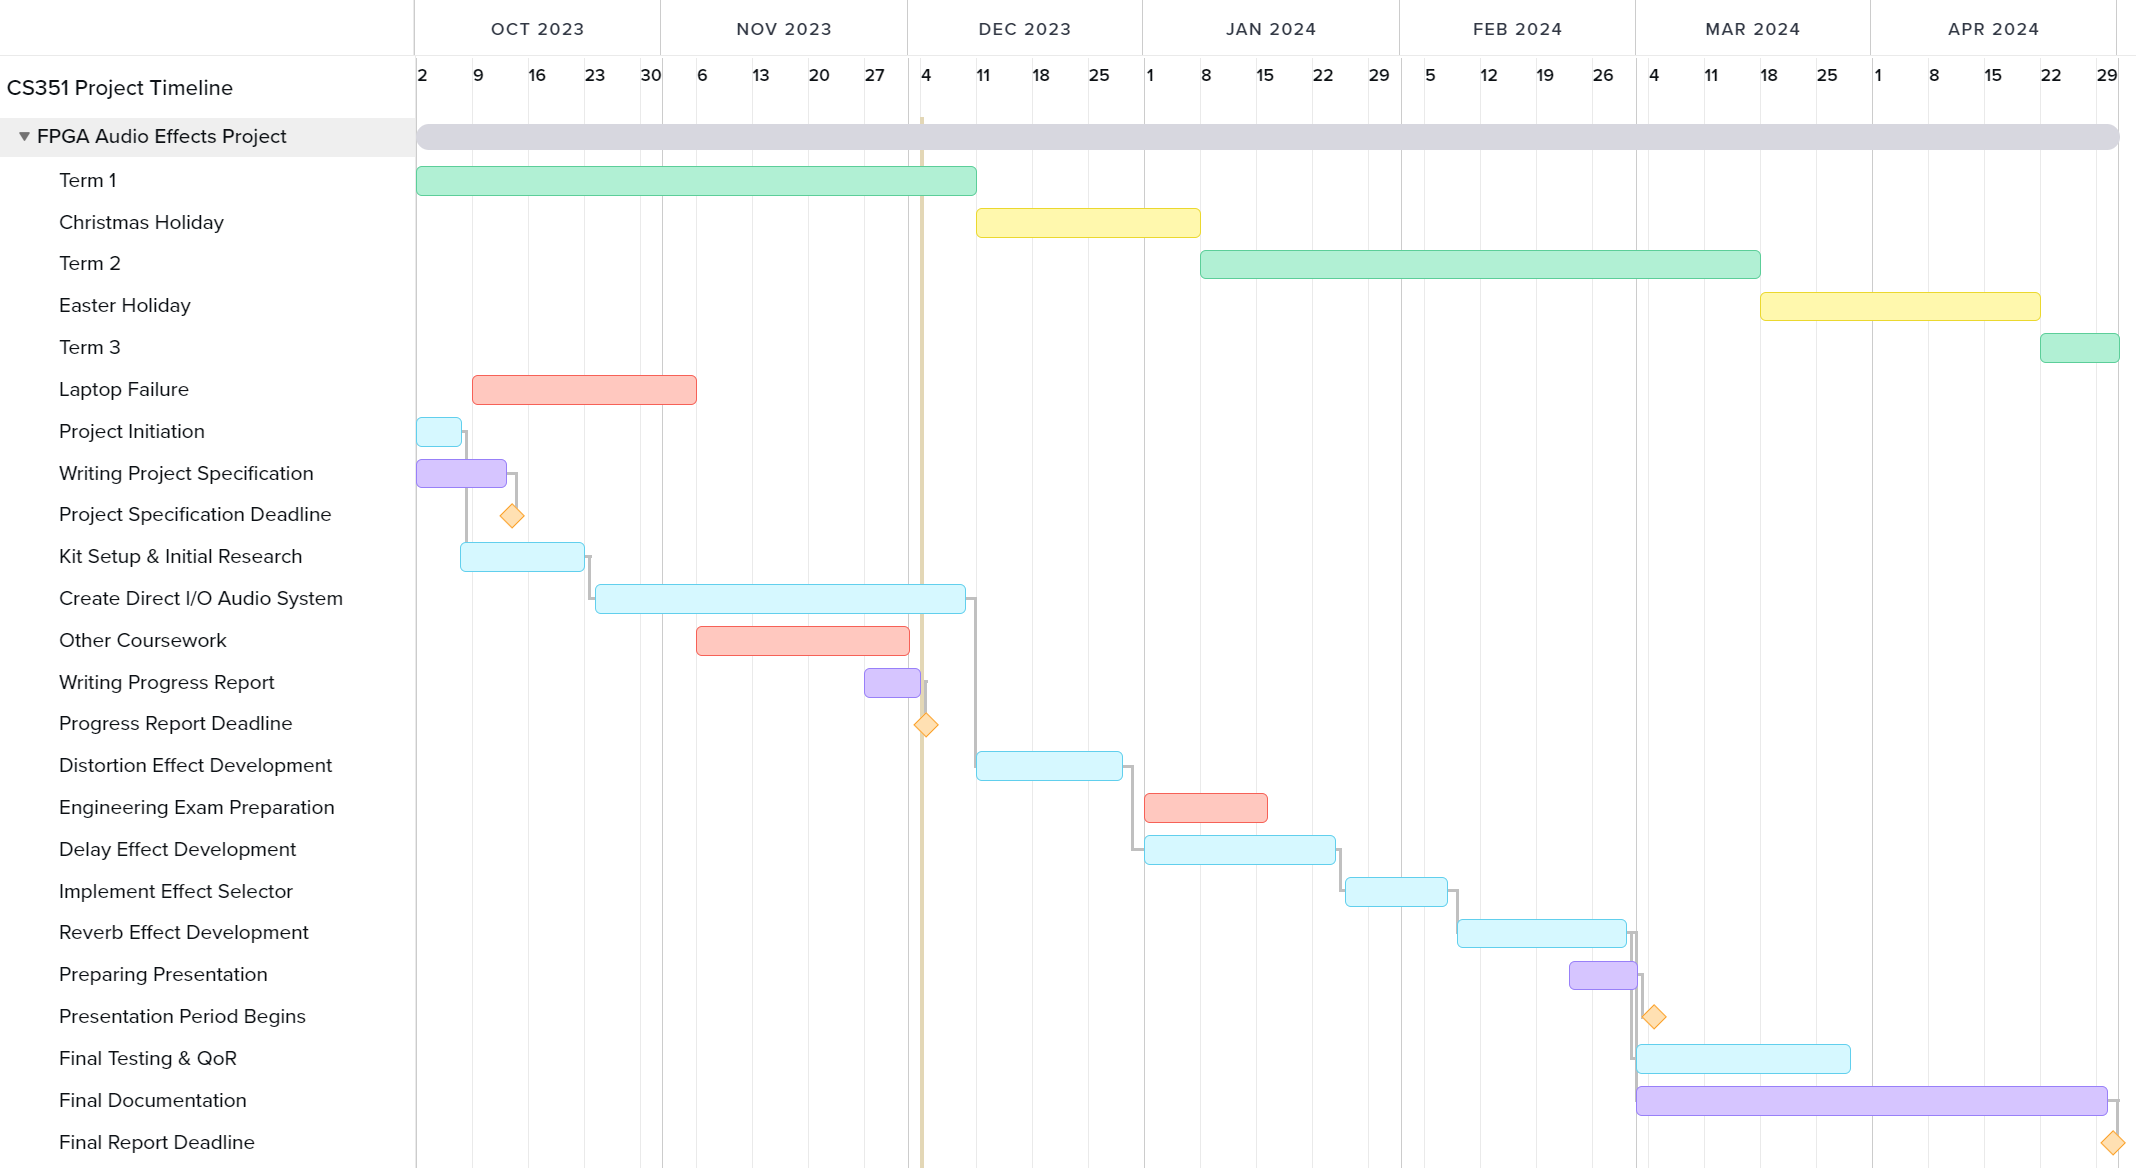
\includegraphics[width=1\linewidth]{progress-report/gantt.png}
    \caption{Gantt Chart of the Updated Timeline}
    \label{fig:gantt}
\end{figure}

The duration of the current task, \textit{Create Direct Audio I/O System} has been increased, resulting in slight delays for the upcoming few activities.

A task has been created for each of the effects found in the \textit{mandatory objectives} list. For the development of each effect, the task consists of research, design, implementation and testing. Since these stages are blended together during development, they are represented as a single activity. As research progressed, the original sorting of the tasks has changed, as it was decided that the effects should be implemented in order of complexity.

Apart from the effects, the project also aims to develop a module that allows real-time toggling of available effects. This is represented in the timeline as the \textit{Implement Effect Selector} task.

\textit{Final testing} and validation for QoR (Quality of Results) is the last task in the development of the product and overlaps with the period designated for completing the Final Report, since most of the results obtained during this stage will be documented in the dissertation.

The chart also illustrates periods where efforts should be focused on written assignments (\textit{Writing Progress Report}, \textit{Preparing Presentation}, etc.), or when other priorities might lead to interruptions in development. However, the durations of each activity have been adjusted accordingly and should not suffer major changes, unless new unpredictable situations occur.